%%%%%%%%%%%%%%%%%%%%%%%%%%%%%%%%%%%%%%%%%
% Programming/Coding Assignment
% LaTeX Template
%
% This template has been downloaded from:
% http://www.latextemplates.com
%
% Original author:
% Ted Pavlic (http://www.tedpavlic.com)
%
% Note:
% The \lipsum[#] commands throughout this template generate dummy text
% to fill the template out. These commands should all be removed when 
% writing assignment content.
%
% This template uses a Perl script as an example snippet of code, most other
% languages are also usable. Configure them in the "CODE INCLUSION 
% CONFIGURATION" section.
%
%%%%%%%%%%%%%%%%%%%%%%%%%%%%%%%%%%%%%%%%%

%----------------------------------------------------------------------------------------
%	PACKAGES AND OTHER DOCUMENT CONFIGURATIONS
%----------------------------------------------------------------------------------------

\documentclass{article}

\usepackage{fancyhdr} % Required for custom headers
\usepackage{lastpage} % Required to determine the last page for the footer
\usepackage{extramarks} % Required for headers and footers
\usepackage[usenames,dvipsnames]{color} % Required for custom colors
\usepackage{graphicx} % Required to insert images
\usepackage{subcaption}
\usepackage{listings} % Required for insertion of code
\usepackage{courier} % Required for the courier font
\usepackage{amsmath}
\usepackage{framed}

% Margins
\topmargin=-0.45in
\evensidemargin=0in
\oddsidemargin=0in
\textwidth=6.5in
\textheight=9.0in
\headsep=0.25in

\linespread{1.1} % Line spacing

% Set up the header and footer
\pagestyle{fancy}
\lhead{\hmwkAuthorName} % Top left header
\chead{\hmwkClass\ (\hmwkClassTime): \hmwkTitle} % Top center head
%\rhead{\firstxmark} % Top right header
\lfoot{\lastxmark} % Bottom left footer
\cfoot{} % Bottom center footer
\rfoot{Page\ \thepage\ of\ \protect\pageref{LastPage}} % Bottom right footer
\renewcommand\headrulewidth{0.4pt} % Size of the header rule
\renewcommand\footrulewidth{0.4pt} % Size of the footer rule

\setlength\parindent{0pt} % Removes all indentation from paragraphs

%----------------------------------------------------------------------------------------
%	CODE INCLUSION CONFIGURATION
%----------------------------------------------------------------------------------------

\definecolor{mygreen}{rgb}{0,0.6,0}
\definecolor{mygray}{rgb}{0.5,0.5,0.5}
\definecolor{mymauve}{rgb}{0.58,0,0.82}

\lstset{ %
  backgroundcolor=\color{white},   % choose the background color
  basicstyle=\footnotesize,        % size of fonts used for the code
  breaklines=true,                 % automatic line breaking only at whitespace
  captionpos=b,                    % sets the caption-position to bottom
  commentstyle=\color{mygreen},    % comment style
  escapeinside={\%*}{*)},          % if you want to add LaTeX within your code
  keywordstyle=\color{blue},       % keyword style
  stringstyle=\color{mymauve},     % string literal style
}

%----------------------------------------------------------------------------------------
%	DOCUMENT STRUCTURE COMMANDS
%	Skip this unless you know what you're doing
%----------------------------------------------------------------------------------------

% Header and footer for when a page split occurs within a problem environment
\newcommand{\enterProblemHeader}[1]{
%\nobreak\extramarks{#1}{#1 continued on next page\ldots}\nobreak
%\nobreak\extramarks{#1 (continued)}{#1 continued on next page\ldots}\nobreak
}

% Header and footer for when a page split occurs between problem environments
\newcommand{\exitProblemHeader}[1]{
%\nobreak\extramarks{#1 (continued)}{#1 continued on next page\ldots}\nobreak
%\nobreak\extramarks{#1}{}\nobreak
}

\setcounter{secnumdepth}{0} % Removes default section numbers
\newcounter{homeworkProblemCounter} % Creates a counter to keep track of the number of problems
\setcounter{homeworkProblemCounter}{0}

\newcommand{\homeworkProblemName}{}
\newenvironment{homeworkProblem}[1][Problem \arabic{homeworkProblemCounter}]{ % Makes a new environment called homeworkProblem which takes 1 argument (custom name) but the default is "Problem #"
\stepcounter{homeworkProblemCounter} % Increase counter for number of problems
\renewcommand{\homeworkProblemName}{#1} % Assign \homeworkProblemName the name of the problem
\section{\homeworkProblemName} % Make a section in the document with the custom problem count
\enterProblemHeader{\homeworkProblemName} % Header and footer within the environment
}{
\exitProblemHeader{\homeworkProblemName} % Header and footer after the environment
}

\newcommand{\problemAnswer}[1]{ % Defines the problem answer command with the content as the only argument
\noindent\framebox[\columnwidth][c]{\begin{minipage}{0.98\columnwidth}#1\end{minipage}} % Makes the box around the problem answer and puts the content inside
}

\newcommand{\homeworkSectionName}{}
\newenvironment{homeworkSection}[1]{ % New environment for sections within homework problems, takes 1 argument - the name of the section
\renewcommand{\homeworkSectionName}{#1} % Assign \homeworkSectionName to the name of the section from the environment argument
\subsection{\homeworkSectionName} % Make a subsection with the custom name of the subsection
\enterProblemHeader{\homeworkProblemName\ [\homeworkSectionName]} % Header and footer within the environment
}{
\enterProblemHeader{\homeworkProblemName} % Header and footer after the environment
}

%----------------------------------------------------------------------------------------
%	NAME AND CLASS SECTION
%----------------------------------------------------------------------------------------

\newcommand{\hmwkTitle}{Assignment 2} % Assignment title
\newcommand{\hmwkDueDate}{Friday, Feb.23, 2018} % Due date
\newcommand{\hmwkClass}{CSC411} % Course/class
\newcommand{\hmwkClassTime}{LEC 5101/0101} % Class/lecture time
\newcommand{\hmwkAuthorName}{Zhongtian Ouyang/Yihao Ni} % Your name

%----------------------------------------------------------------------------------------
%	TITLE PAGE
%----------------------------------------------------------------------------------------

\title{
\vspace{2in}
\textmd{\textbf{\hmwkClass:\ \hmwkTitle}}\\
\normalsize\vspace{0.1in}\small{Due\ on\ \hmwkDueDate}\\
\vspace{0.1in}
\vspace{3in}
}

\author{\textbf{\hmwkAuthorName}}
\date{} % Insert date here if you want it to appear below your name

%----------------------------------------------------------------------------------------

\begin{document}

\maketitle
\clearpage
%----------------------------------------------------------------------------------------
%	PROBLEM 1
%----------------------------------------------------------------------------------------

% To have just one problem per page, simply put a \clearpage after each problem

\begin{homeworkProblem}

\noindent \textit{Dataset description}\\

The pictures are loaded from mnist\_all.mat and combined using the showDigits() function. Each line is a digit from 0 to 9. Based on those 10 images for each digit, this dataset includes various styles of writing those digits.  Most of the images are great, but some of those images consists of something unrelated. For example, the third image of '1' has a ':' next to it, and the first image of '5' has a meaningless circle.

\begin{figure*}[!ht]
 \centering
    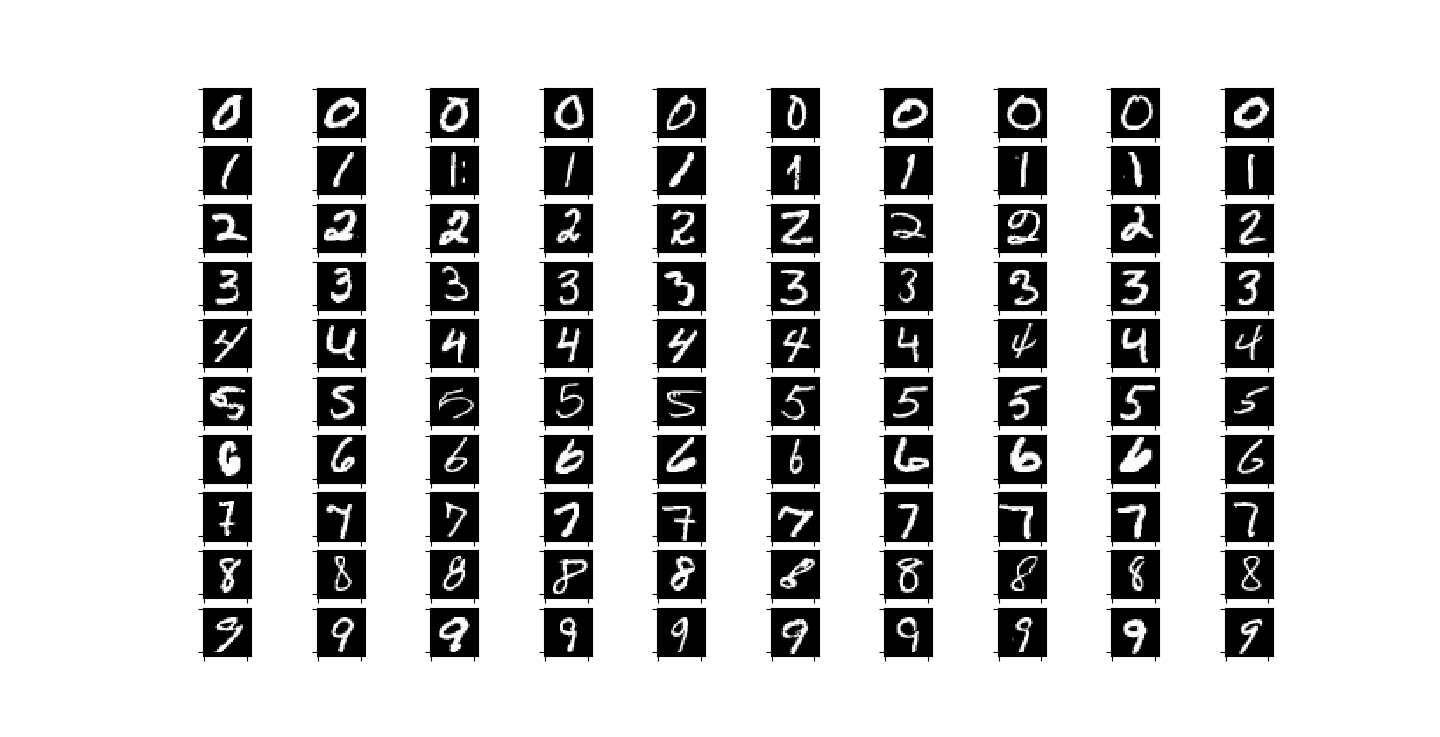
\includegraphics[scale=0.45]{digits.png}
    \caption{10 random images for each digit}
    \label{fig:digits}
\end{figure*}


\end{homeworkProblem}
\clearpage
%----------------------------------------------------------------------------------------
%	PROBLEM 2
%----------------------------------------------------------------------------------------

\begin{homeworkProblem}
\noindent \textit{Neural network}\\

The function forward\_p2 first compute $o$ using the formula given, then compute the softmax using the softmax function. The requirements of the inputs are included in the comment. The code is as follows:

\begin{framed}
\begin{lstlisting}[language=python]
def softmax(y):
   '''Return the output of the softmax function for the matrix of output y. y
   is an N x M matrix where N is the number of outputs for a single case, and M
   is the number of cases'''
   return exp(y)/tile(sum(exp(y),0), (len(y),1))

def forward_p2(x, w, b):
   '''the input x should be 784 x n, the input w should be 784 x 10, the input b
    should be 10 x 1 in our case
   '''
   Os = dot(w.T, x) + b
   result = softmax(Os)
   return result
\end{lstlisting}
\end{framed}



\end{homeworkProblem}
\clearpage

%----------------------------------------------------------------------------------------
%	PROBLEM 3
%----------------------------------------------------------------------------------------

\begin{homeworkProblem}
\noindent \textit{Compute the gradient}
\\Part(a):\\
The cost function for s sample cases:
$$C = \sum_{s}(-  \sum_{k}y_{k}^{s} log p_{k}^{s} )$$
Apply the chain rule to get the gradient of the cost function with respect to the weights:

$$\frac{\partial C}{\partial W_{ij}} = \frac{\partial C}{\partial o_{i}} \frac{\partial o_{i}}{\partial w_{ij}} = \sum_{s} (p_{i}^{s} - y_{i}^{s})x_{j}^{s}$$

Where $\frac{\partial C}{\partial o_{i}}$ is computed as follows:

\begin{equation}
\begin{split}
\frac{\partial C}{\partial o_{i}} & = \frac{\partial C}{\partial p_{i}} \frac{\partial p_{i}}{\partial o_{i}} + \sum_{k \neq i}\frac{\partial C}{\partial p_{k}} \frac{\partial p_{k}}{\partial o_{i}} \\
& = -\frac{y_{i}}{p_{i}} p_{i}(1 - p_{i}) - \sum_{k \neq i} \frac{y_{k}}{p_{k}} (-p_{i}p_{k}) \\
& = y_{i}p_{i} - y_{i} + \sum_{k \neq i} p_{i}y_{k} \\
& = \sum_{k} p_{i}y_{k} - y_{i}\\
& = p_{i} - y_{i}
\end{split}
\end{equation}

$\frac{\partial o_{i}}{\partial w_{ij}}$ simply equals to:
$$\frac{\partial o_{i}}{\partial w_{ij}} =  \frac{\partial}{\partial w_{ij}} \sum_{s}(w_{i0}x_{0}^{s}+w_{i1}x_{1}^{s}+ ...+ w_{ij}x_{j}^{s}+ ... + b) =\sum_{s} x_{j}^{s}$$

Where $i = 0,...,9$ and $j = 0,...,783$ in our case, s is the sample size. Therefore $\frac{\partial C}{\partial W_{ij}}$ has a dimension of $10*784$.\\

Part(b):\\
The code for computing the gradients is as follows:

\begin{framed}
\begin{lstlisting}[language=python]
def softmax(y):
   '''Return the output of the softmax function for the matrix of output y. y
   is an N x M matrix where N is the number of outputs for a single case, and M
   is the number of cases'''
   return exp(y)/tile(sum(exp(y),0), (len(y),1))

def forward_p2(x, w, b):
   '''the input x should be 784 x n, the input w should be 784 x 10, the input b
    should be 10 x 1 in our case
   '''
   Os = dot(w.T, x) + b
   result = softmax(Os)
   return result

def grad_p3(x, w, b, y):
    '''
    return the gradient of weights and the gradient of biases
    '''
    p = forward_p2(x, w, b)
    dc_do = p - y
    return np.dot(dc_do, x.T).T, np.dot(dc_do, np.ones((x.shape[1], 1)))
\end{lstlisting}
\end{framed}

Parameter dc\_do in function grad\_p3 is $\frac{\partial C}{\partial o}$ in part(a). Following is obtained by approximating the gradient at several coordinates using finite differences:

\begin{framed}
when h = 0.1:\\
The sum of the absolute value of difference for weight is 0.11572252765064116\\
The average of the absolute value of difference for weight is 1.4760526486051168e-05\\
The sum of the absolute value of difference for bias is 0.0005599162912244271\\
The average of the absolute value of difference for bias is 5.599162912244271e-05\\~\\
When h = 0.001:\\
The sum of the absolute value of difference for weight is 1.1595024297009595e-05\\
The average of the absolute value of difference for weight is 1.4789571807410197e-09\\
The sum of the absolute value of difference for bias is 5.597965579973163e-08\\
The average of the absolute value of difference for bias is 5.597965579973163e-09\\~\\
When h = 0.0001:\\
The sum of the absolute value of difference for weight is 3.1475914028065034e-06\\
The average of the absolute value of difference for weight is 4.0147849525593155e-10\\
The sum of the absolute value of difference for bias is 3.5902092410111663e-09\\
The average of the absolute value of difference for bias is 3.5902092410111663e-10
\end{framed}

It is clear that when h gets smaller, the difference gets smaller as well. Therefore if h gets arbitrarily small, the difference approaches zero, which indicates our gradient is computed correctly.
\end{homeworkProblem}
\clearpage
%----------------------------------------------------------------------------------------
%	PROBLEM 4
%----------------------------------------------------------------------------------------

\begin{homeworkProblem}
\noindent \textit{Gradient descent without momentum}\\
The sets are obtained through the get\_sets() function. To get the validation and training set. we shuffled the training set from the data set and use the first 4000 as the training set and the following 1000 as the validation set. For the test set, we shuffle the set from data and take the first 850 cases.\\
We had tried to initialize the weight with random numbers, normal distributed normal numbers and all zeros. We choose the weight to be instialized as all zeros because that would keep the weights correspond irrelevant pixels, which are the pixels that are always black in all cases, keep at 0. While the weights for relevant point would have a non zero weight and thus become non-zero.\\
We pick 0.00003 as learning rate. Bigger values such as 0.01 will lead to overflow, and values like 0.0001 will cause the cost to increase in some iterations ,showing that the weight is moving back and forth around the center. The full learning curve runs for 1500 iteration. To make it clear, we also include the curve with only 30 iterations. Following is the curve.\\
NOTICE: the lines are pretty much identical. But if observed carefully, you can see three seperated lines.


\begin{figure*}[!ht]
\begin{subfigure}{1\textwidth}
 \centering
  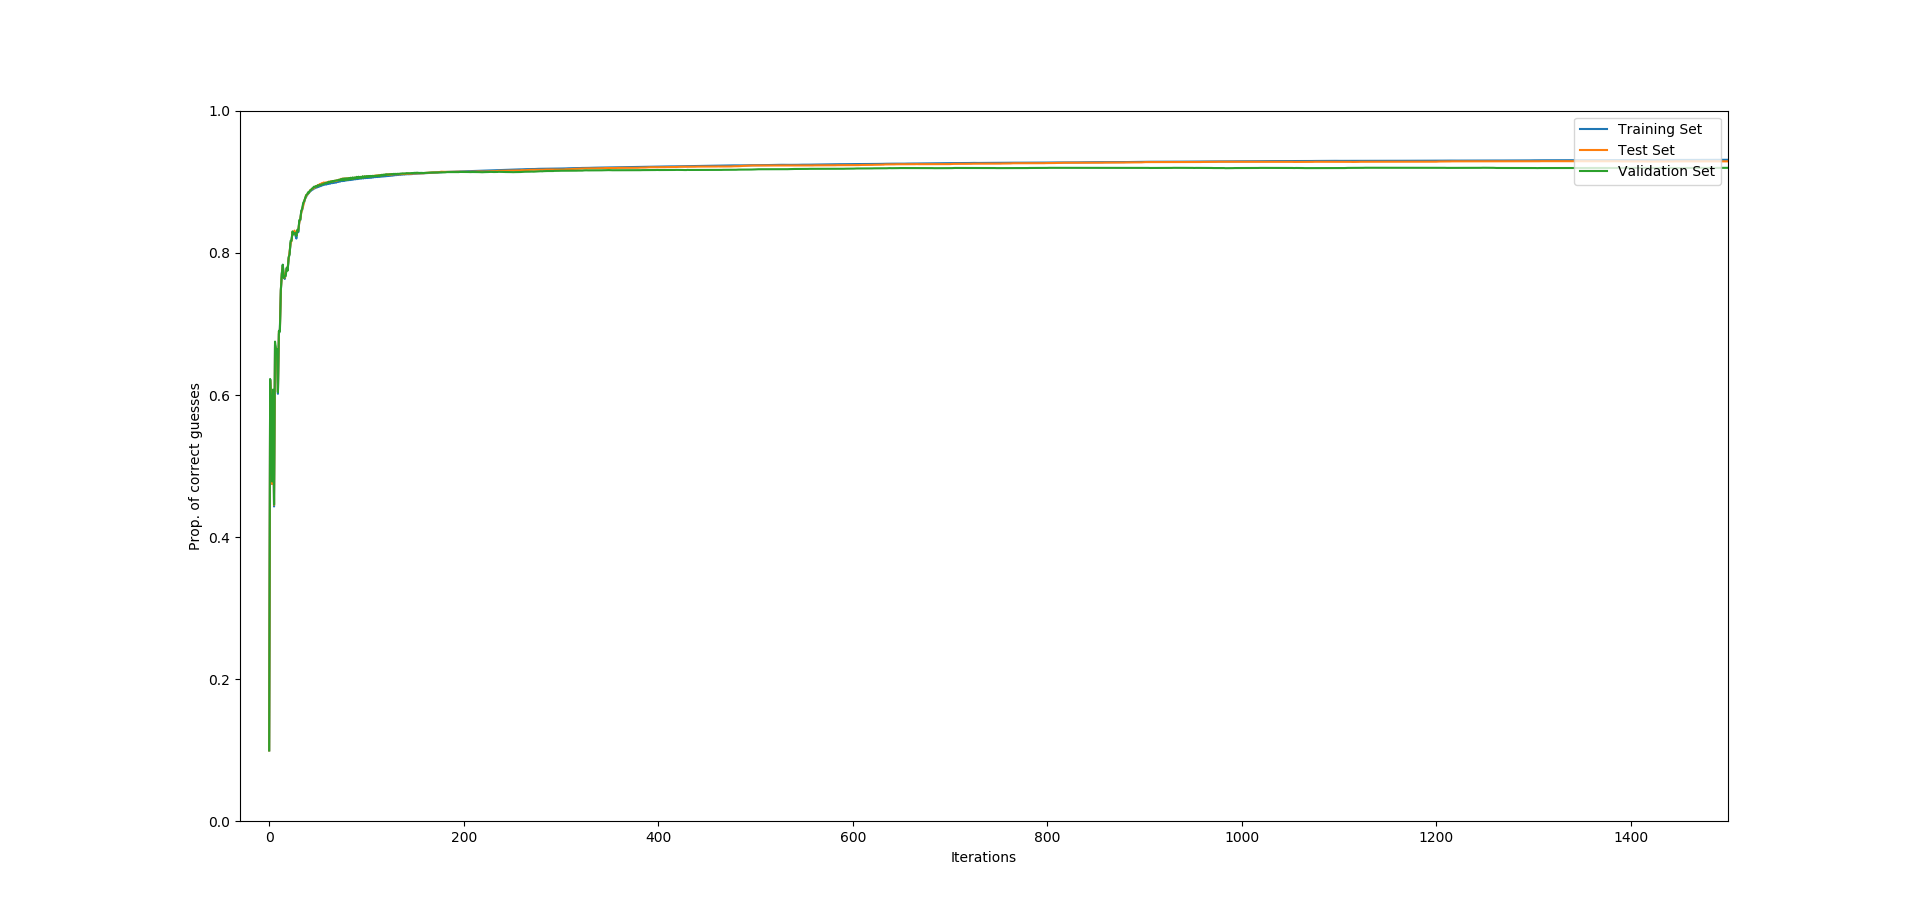
\includegraphics[width=.8\linewidth]{p4_learning.png}
  \caption{Full learning curve}
  \label{fig:sfig1}
\end{subfigure}
\begin{subfigure}{1\textwidth}
 \centering
  \includegraphics[width=.8\linewidth]{P4_learning_30.png}
  \caption{learning curve for first 30 iterations}
  \label{fig:sfig2}
\end{subfigure}%
\caption{Part4}
\label{fig:p4}
\end{figure*}

The weights connecting to each output are as follows:


\begin{figure}[!ht]
\centering
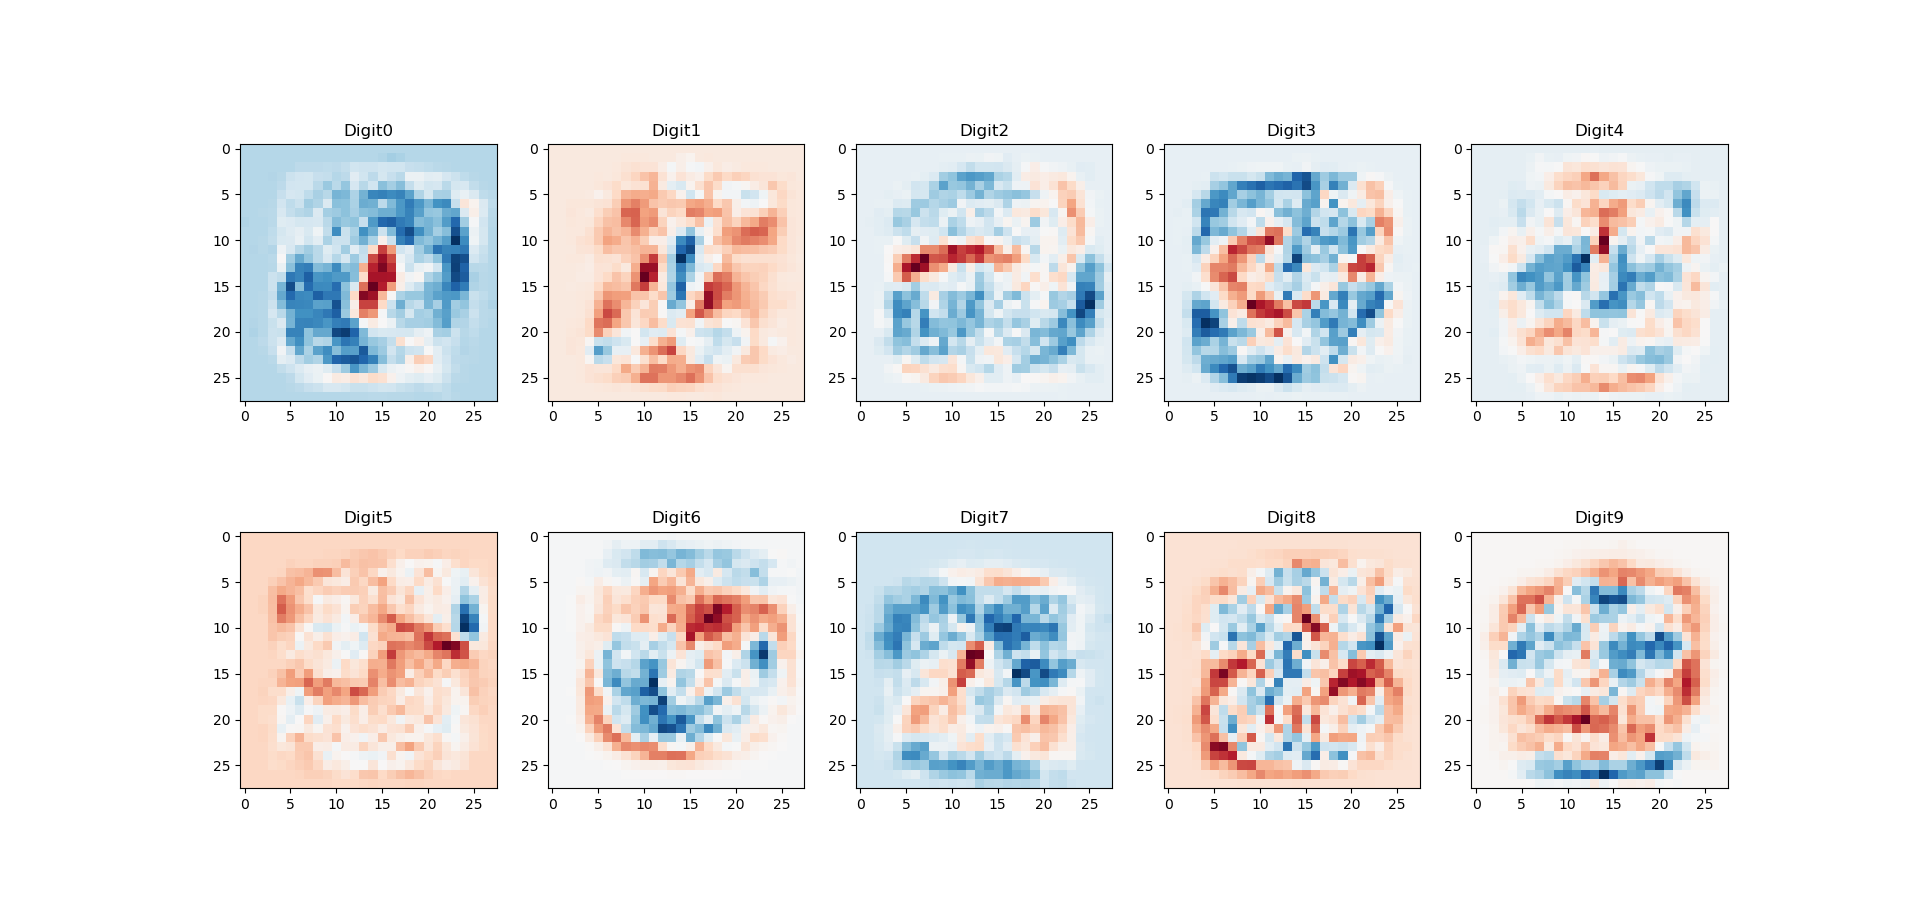
\includegraphics[width=1\linewidth]{p4_weight.png}
\caption{Visualization of weights}
\label{fig:p4w}
\end{figure}



\end{homeworkProblem}
\clearpage

%----------------------------------------------------------------------------------------
%	PROBLEM 5
%----------------------------------------------------------------------------------------

\begin{homeworkProblem}
\noindent \textit{Gradient descent with momentum}\\
We use the same learning rates and iteration as problem 4. And we use 0.9 as the gamma value. All the sets are the same as previous\\
Following is the code that performs gradient descent with momentum and the learning curves. We can observe that although the full learning curve looks similar to the one without momentum, if we focus on the first 30 iterations, the one with momentum is much more smooth and more effecient. It reaches 0.8 with only about 5 iterations, while the one without momentum needs over 10 iterations. And the smooth curve shows that we are keep running toward the center.

\begin{framed}
\begin{lstlisting}[language=python]
def grad_descent_m(f, df, x, y, init_t, init_b, alpha, gamma, max_iter, test,
                   t_answer, validation, v_answer, plotCurve=True):
    EPS = 1e-5  # EPS = 10**(-5)
    prev_t = init_t - 10 * EPS
    t = init_t.copy()
    prev_b = init_b - 10 * EPS
    b = init_b.copy()
    vt = 0
    vb = 0
    iter = 0
    perfomance_x = [perform(x, t, b, y)]
    perfomance_t = [perform(test, t, b, t_answer)]
    perfomance_v = [perform(validation, t, b, v_answer)]
    iterations = [0]
    print('Doing gradient Descent')
    while (np.linalg.norm(t - prev_t) + np.linalg.norm(
                b - prev_b)) > EPS and iter < max_iter:
        prev_t = t.copy()
        prev_b = b.copy()
        grad_t, grad_b = df(x, t, b, y)
        vt = gamma * vt + alpha * grad_t
        vb = gamma * vb + alpha * grad_b
        t -= vt
        b -= vb
        if iter % 100 == 0:
            print("Iter", iter)
            print("f(x) = %.2f" % (f(forward_p2(x, t, b), y)))
            # print("Gradient: ", df(x, t, b, y), "\n")
        if plotCurve:
            perfomance_x.append(perform(x, t, b, y))
            perfomance_t.append(perform(test, t, b, t_answer))
            perfomance_v.append(perform(validation, t, b, v_answer))
            iterations.append(iter + 1)
        iter += 1
    if plotCurve:
        plt.plot(iterations, perfomance_x)
        plt.plot(iterations, perfomance_t)
        plt.plot(iterations, perfomance_v)
        plt.legend(['Training Set', 'Test Set', 'Validation Set'],
                   loc='upper right')
        plt.axis([-30, max_iter, 0, 1])
        plt.ylabel('Prop. of correct guesses')
        plt.xlabel('Iterations')
        plt.show()
    print('Final Cost is ' + format(f(forward_p2(x, t, b), y), '.2f'))
    return t, b
\end{lstlisting}
\end{framed}

\begin{figure*}[!ht]
\begin{subfigure}{1\textwidth}
 \centering
  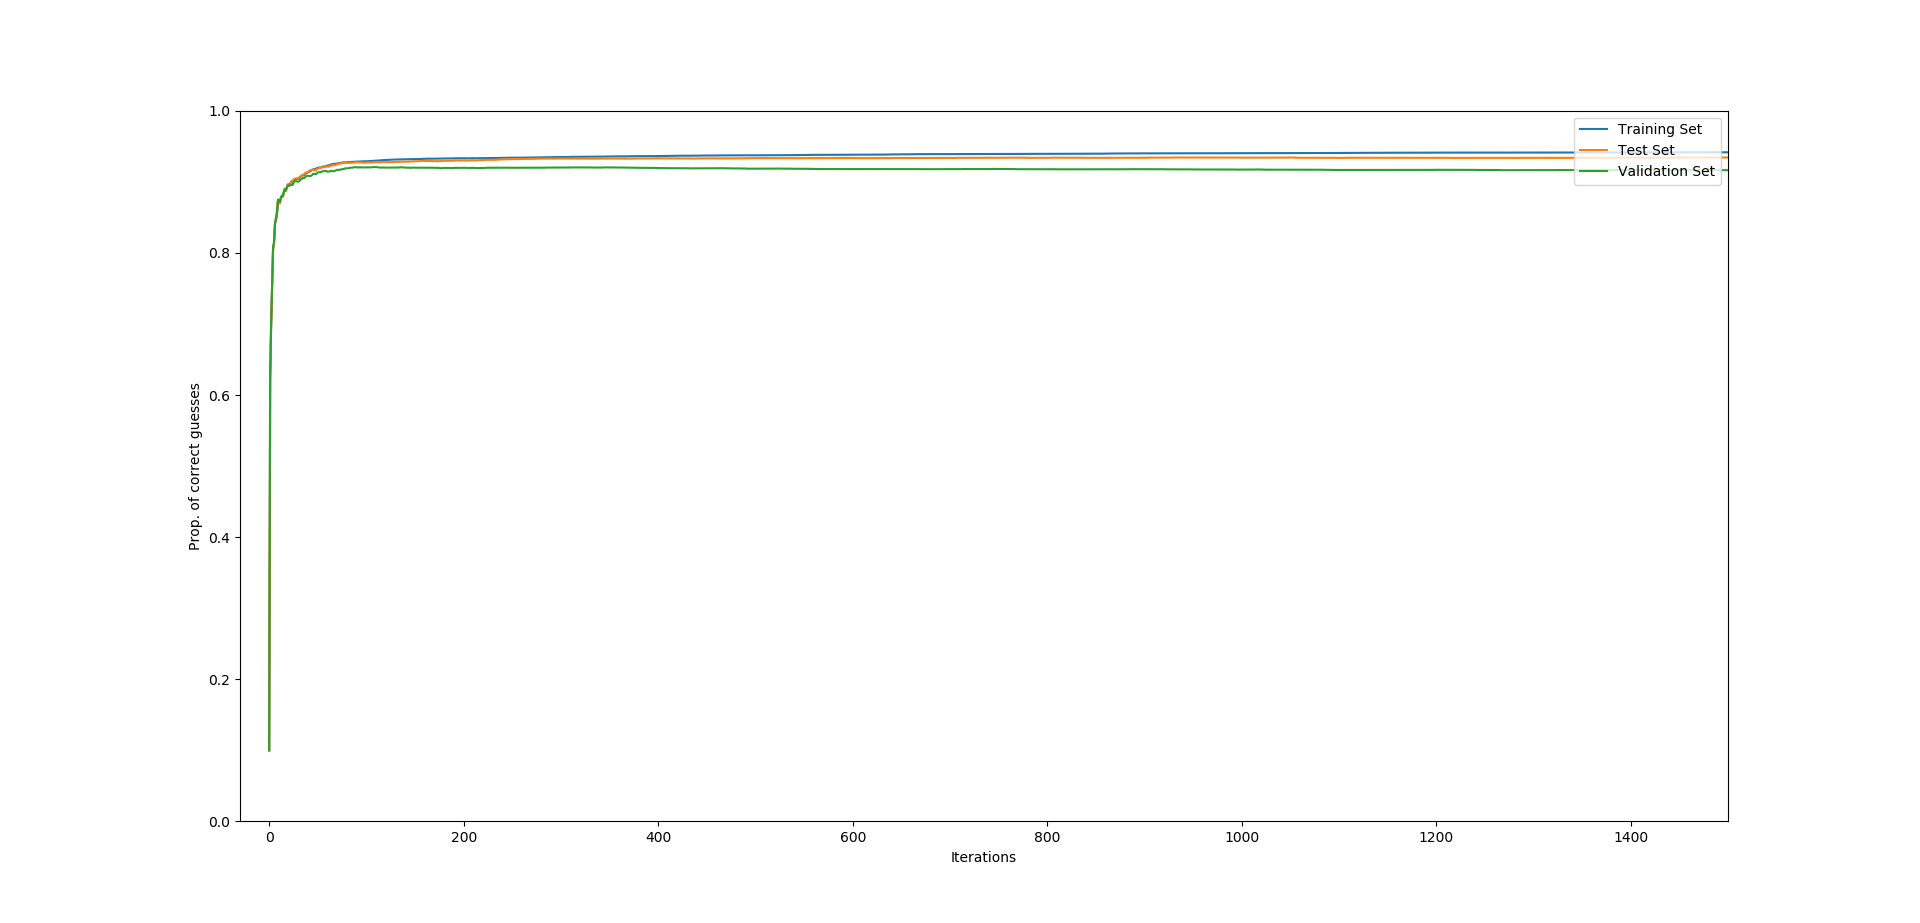
\includegraphics[width=.8\linewidth]{p5_learning.png}
  \caption{Full learning curve}
  \label{fig:sfig1}
\end{subfigure}
\begin{subfigure}{1\textwidth}
 \centering
  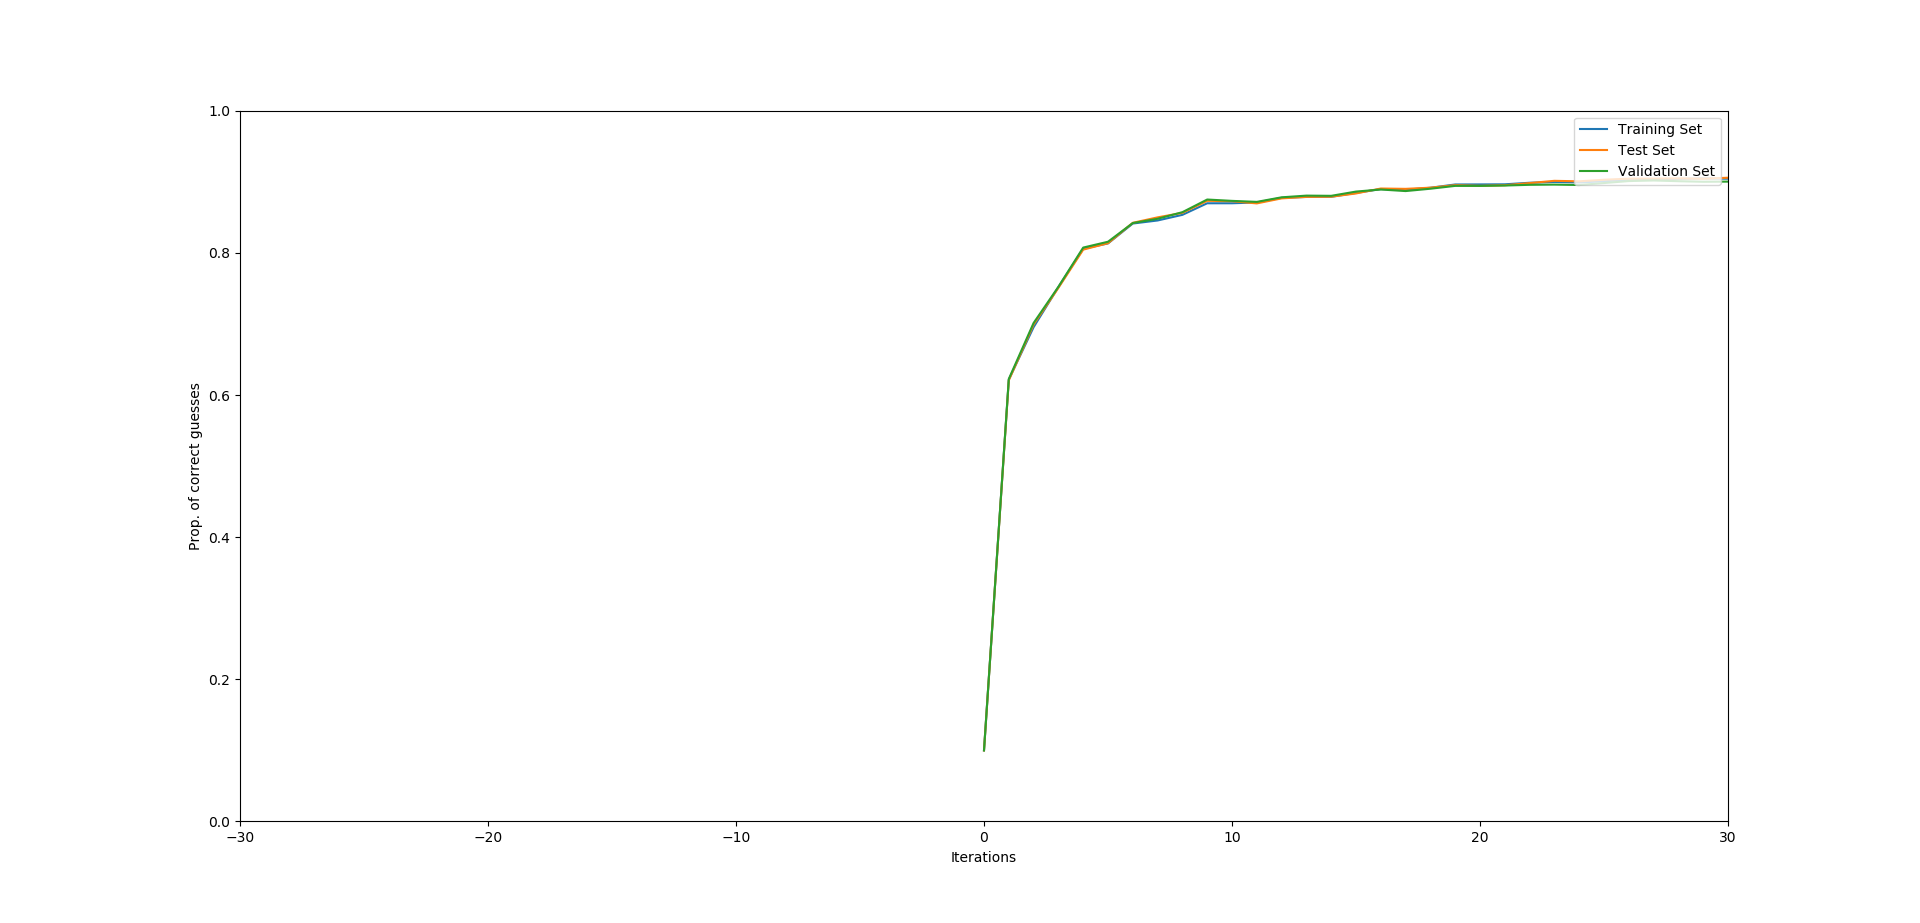
\includegraphics[width=.8\linewidth]{p5_learning_30.png}
  \caption{learning curve for first 30 iterations}
  \label{fig:sfig2}
\end{subfigure}
\caption{Part5}
\label{fig:p5}
\end{figure*}

\end{homeworkProblem}
\clearpage
%----------------------------------------------------------------------------------------
%	PROBLEM 6
%----------------------------------------------------------------------------------------
\begin{homeworkProblem}
\noindent \textit{Momentum performance}

Part(a)\\
Following is the contour plot of the cost function from Part 5. The two weights are chosen to be $11*28+11$ and $17*28+17$, since pixels in the center of the image is more likely to be part of the digit, and thus does not has weight zero. The center is around (0.5, -0.5).

\begin{figure}[!ht]
\centering
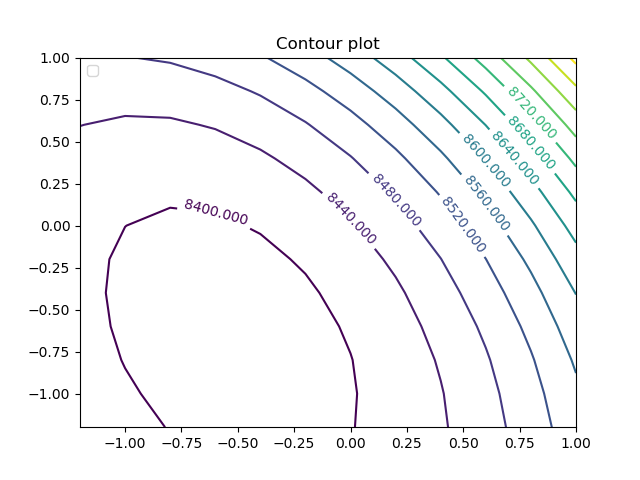
\includegraphics[width=1\linewidth]{p6a.png}
\caption{contour plot of the cost function}
\label{fig:p6a}
\end{figure}
\clearpage
Part(b)(c)(d)\\

Starting point is (0.8, 0.8). Learning rate is chosen to be 0.003 for both trajectories, 100 times as it was in Part5, this is because the max iteration here is just 20 to visualize all points on the graph. Gamma is 0.7, smaller than that in Part(5), since larger gamma such as 0.9 chosen in Part(5) would make it cross the center point to the lower left side, which is too much. Green dots are gradient descent with momentum, while yellow ones are that without momentum.
\begin{figure*}[!ht]
\centering
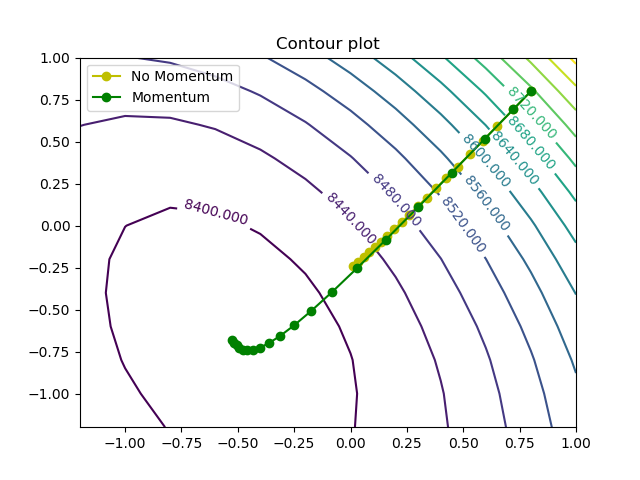
\includegraphics[width=1\linewidth]{p6bc.png}
\caption{contour plot of the cost function with two trajectories}
\label{fig:p6bc}
\end{figure*}
It can be visualized in this graph that the green dots approaches the center much faster than yellow dots do. This is because when we use gradiant descent with momentum, each step is increased with the amount calculated by last step, so that it approaches the center point faster.\\
\clearpage
Part(e):\\
This is an example of bad choice of settings and weights. The two chosen pixels are the upper-left one and the bottom-right one, in the corners, which is more likely to have nothing to do with the digits. It can be observed that nothing is on the graph except for a green point (the yellow one might be covered by it). The contour line does not appear since all points on the graph have a same (or similar) value, thus no contour lines to be shown.

\begin{figure*}[!ht]
\centering
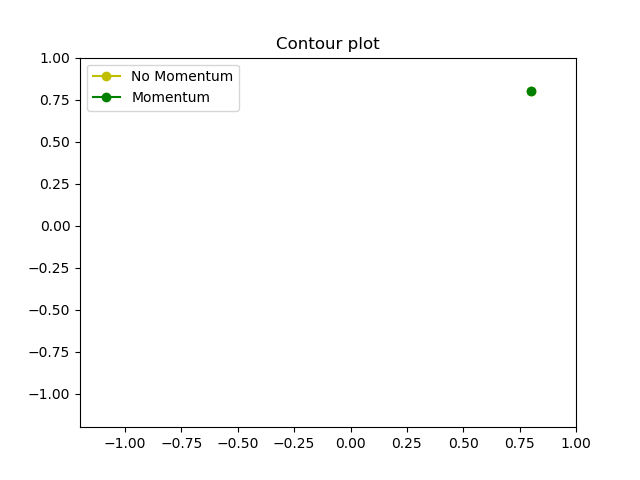
\includegraphics[width=1\linewidth]{p6e.png}
\caption{Inappropriate choise of settings and weights}
\label{fig:p6e}
\end{figure*}
\end{homeworkProblem}
\clearpage
%----------------------------------------------------------------------------------------
%	PROBLEM 7
%----------------------------------------------------------------------------------------
\begin{homeworkProblem}
\noindent \textit{Backpropagation for a network with NK neurons}
\\For a network with N layers each of which contains K neurons, there are K*N neurons in total.\\
Cost for fully vectorized backpropagation:\\
Using the cache values, the derivative with respect to each weight between layers can be calculated by just one matrix multiplication. Given each layer contains K neurons, the matrices are K by K. Multiply two K by K matrices has complexity $O(n^{3})$. Therefore, the complexity of vectorized backpropogation is $O(NK^{3})$.
Cost for computing gradient individually:\\
For a specific weight into layer N (the upper one) the complexity would be O(1), and for all the weights the complexity is $O(K^{2})$, and for layer N-1 (the second upper one) the complexity would be $O(n^{3})$.  Since we are computing those values individually, those complexity have to be summed up to get the total cost, and it would be:
$O(K^{2}) + O(K^{3}) + ... +O(K^{N})$, which is complexity $O(K^{N})$.\\
For large values of K and N, using fully vectorized backpropagation change the complexity from $O(NK^{3})$ to $O(K^{N})$, which is a big improvemnet.

\end{homeworkProblem}
\clearpage
%----------------------------------------------------------------------------------------
%	PROBLEM 8
%----------------------------------------------------------------------------------------
\begin{homeworkProblem}
\noindent \textit{Single-hidden-layer fully-connected network with pytorch}\\
The performance of the network on test set is 87.29\%\\
The images are downloaded and cropped to 32 * 32 using get\_data.py.\\
The network has a bottom layer with 3072 units, a top layer with 6 units and one fully connected hidden layer with 18 units. The activation function for the hidden layer is the Tahn function. I had also tried ReLU and Sigmoid as activation function, but they both yield worse results.\\
The cost function I used is the CrossEntropyLoss function. And I use Adam as an optimizer.\\
The weights for the two linear layers are initialized randomly with normal distribution. At first, I set the variance to 0.1. Later I find out that variance is too larget, causing some weights to be too far away from the ideal with almost zero gradient, so I changed the variance to 0.001 and improved my performance by about 5\%\\
The samples are divided into minibatches. I first choose batch size to be 10, and gradually increase it to 50, 75, 100, 200. Batch size 100 yields the best result among the choices.  The learning rate is 1e-3. I stop the training at 1000 epochs because more epochs would overfit the model too much and decrease the performance on the validation set.\\
I choose 18 neurons initially, which are supposed to match to the front, left side and right side of the 6 actors.(Though this doesn't seem to be the case from part 9 result). And with some testing using 12,18,24,30 neurons, both 18 and 24 yield the best result on the validation set. And since 18 neuron is less expensive to calculate, I choose to use 18 neurons.\\
Also, to avoid overfitting, I applied L2 regularization by setting the weight\_decay for Adam optimizer to 1e-5
\begin{figure}[!ht]
\centering
\includegraphics[width=1\linewidth]{p8.png}
\caption{Learning curve}
\label{fig:p8}
\end{figure}
\end{homeworkProblem}
\clearpage
%----------------------------------------------------------------------------------------
%	PROBLEM 9
%----------------------------------------------------------------------------------------
\begin{homeworkProblem}
\noindent \textit{Useful neurons to classify two specific actors}\\
The two actors I choose are Bracco and Baldwin. Below are the visualization of the weights of the 5 most useful neurons to classify each actor. Here are the steps to find out the most useful neurons:\\
1. Get the weights w of the 6-neuron top layer of the network. The shape of the weights would be 6 * number of hidden neurons in our case.
2.  Each row of w would be how much each hidden-layer neuron contribute to classifying a specific actor. For example, The first row would be for the actor with y being [1, 0, 0, 0, 0, 0], Bracco in my case. And the value at index k of that row shows how the kth neuron contribute to classifying a picture as Bracco. If the value is positive, it means activating the neuron suggest that this is a picture of Bracco. Vice Versa.\\
3. Find the indexes of the five largest numbers in the actors' row. A greater number means the evidence is stronger.\\
4. Visualize the weights of the neurons in the hidden layer with the five indexes we find in previous step.
\begin{figure*}[!ht]
\begin{subfigure}{1\textwidth}
 \centering
  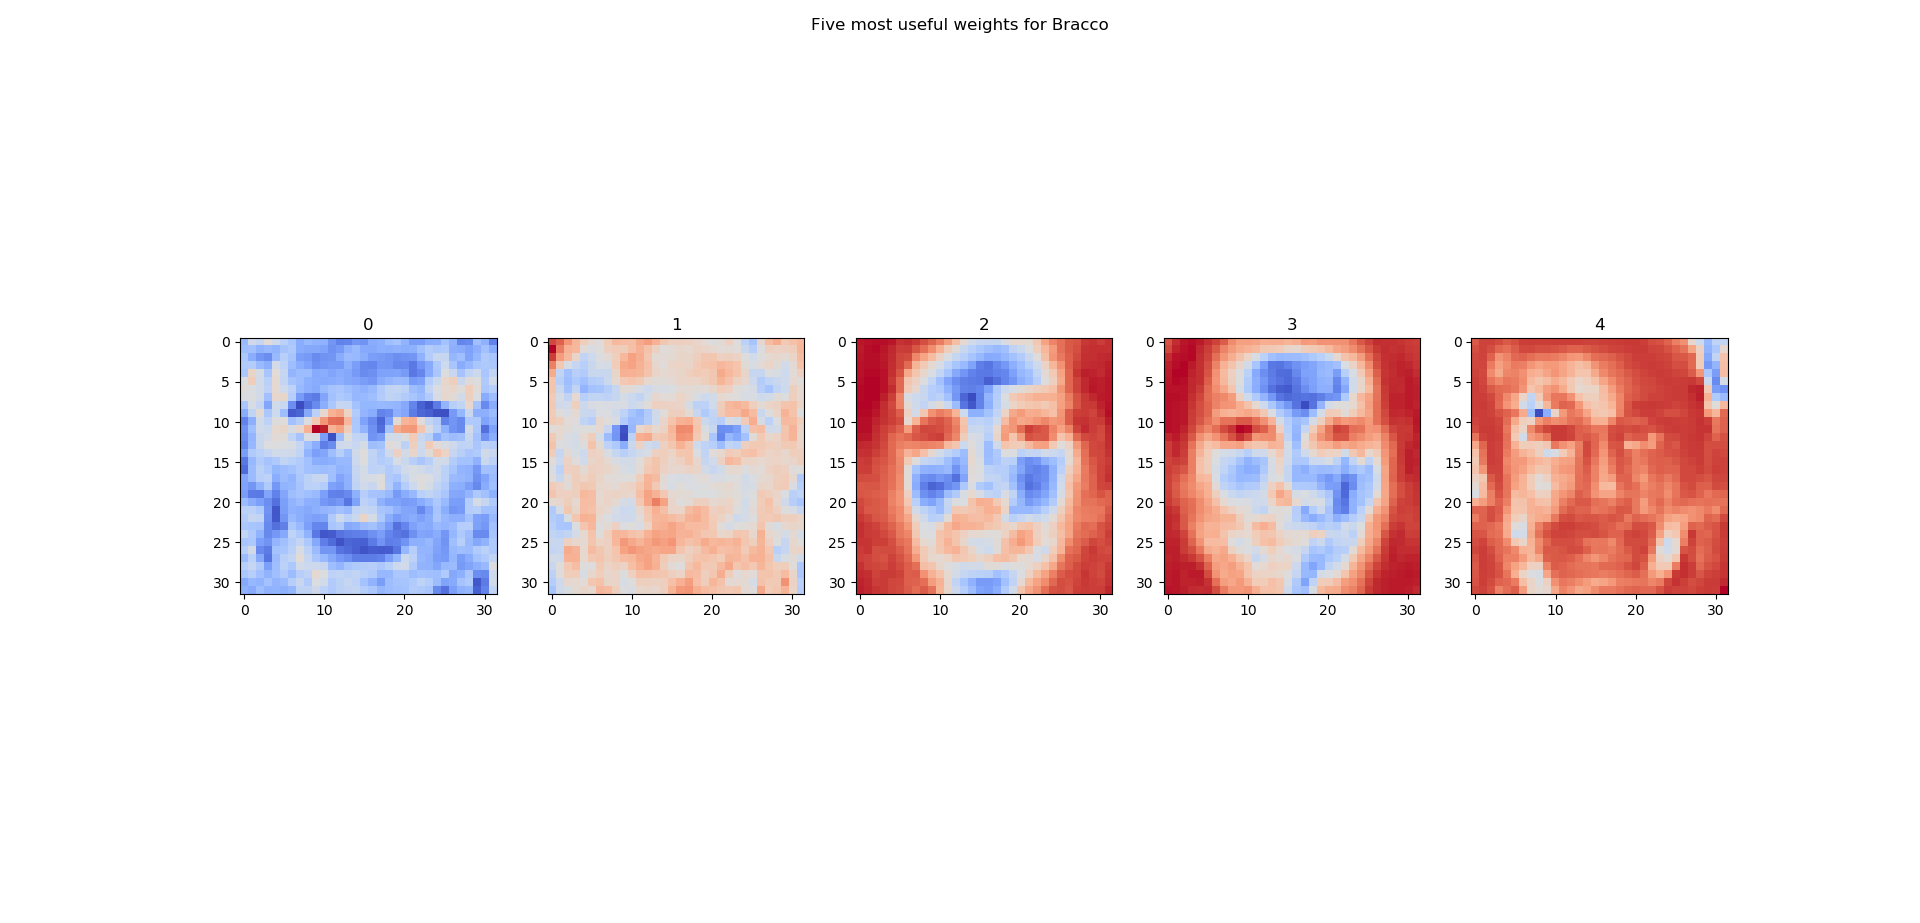
\includegraphics[width=.8\linewidth]{p9_bracco.png}
  \caption{Neurons supporting Bracco}
  \label{fig:sfig1}
\end{subfigure}
\begin{subfigure}{1\textwidth}
 \centering
  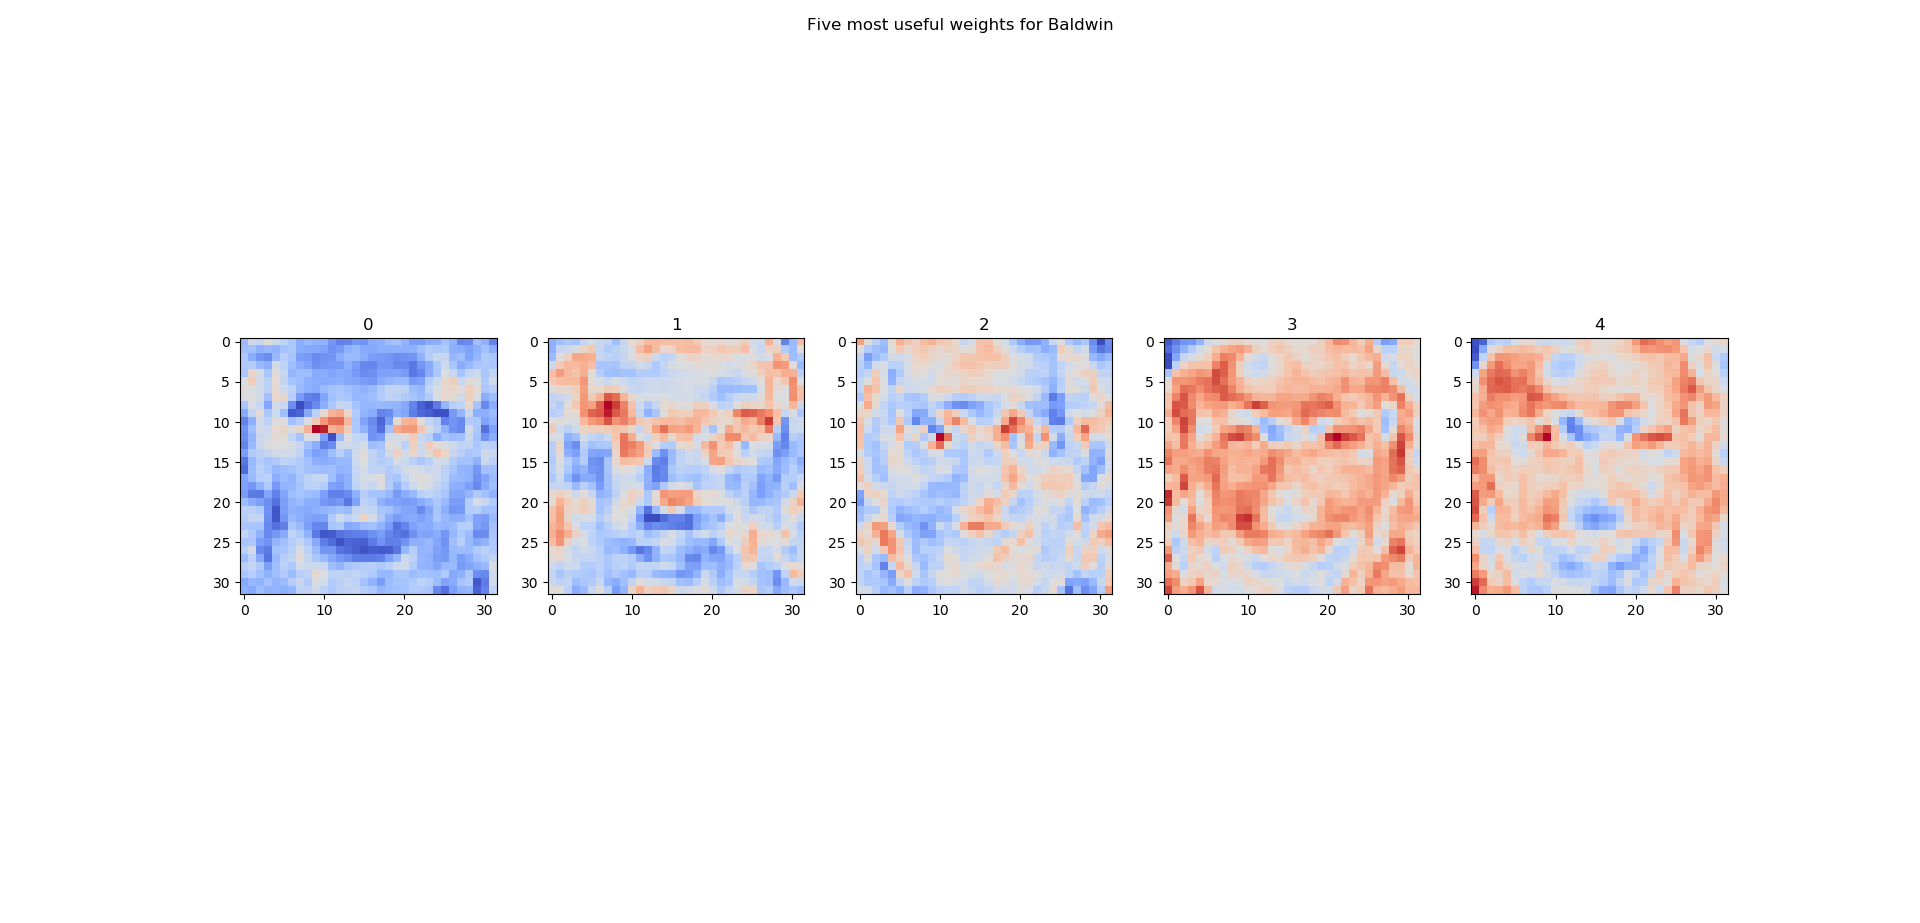
\includegraphics[width=.8\linewidth]{p9_baldwin.png}
  \caption{Neurons supporting Baldwin}
  \label{fig:sfig2}
\end{subfigure}%
\caption{Part9}
\label{fig:p9}
\end{figure*}
\end{homeworkProblem}
\clearpage
%----------------------------------------------------------------------------------------
%	PROBLEM 10
%----------------------------------------------------------------------------------------
\begin{homeworkProblem}
\noindent \textit{Single-hidden-layer fully-connected network with pytorch}

\end{homeworkProblem}
\clearpage
%----------------------------------------------------------------------------------------

\end{document}
